%----------------------------------------------------------------------------------------
%    PACKAGES AND THEMES
%----------------------------------------------------------------------------------------

\documentclass[aspectratio=169,xcolor=dvipsnames]{beamer}
\usetheme{SimpleDarkBlue}

\usepackage{hyperref}
\usepackage{graphicx} % Allows including images
\usepackage{booktabs} % Allows the use of \toprule, \midrule and \bottomrule in tables

%----------------------------------------------------------------------------------------
%    TITLE PAGE
%----------------------------------------------------------------------------------------

\title{Human-Benchmark}
\subtitle{2 Laboratorinis}

\author{Adrian, Arnas, Darius, Tadas}

\institute
{
    Matematikos ir informatikos fakultetas \\
    Vilniaus universitetas % Your institution for the title page
}
% \date{\today} % Date, can be changed to a custom date 

%----------------------------------------------------------------------------------------
%    PRESENTATION SLIDES
%----------------------------------------------------------------------------------------

\begin{document}

\begin{frame}
    % Print the title page as the first slide
    \titlepage
\end{frame}

\begin{frame}{Apžvalga}
    % Throughout your presentation, if you choose to use \section{} and \subsection{} commands, these will automatically be printed on this slide as an overview of your presentation
    \tableofcontents
\end{frame}

\section{Reikalavimai}

\begin{frame}{Reikalavimai (1/2)}
    \textbf{Pagrindinės kategorijos:}
    \begin{itemize}
        \item \textbf{Jungiamumas:} Sklandus bendravimas (WebSocket, kelių žaidėjų valdymas, API sąveikos).
        \item \textbf{Prieinamumas:} Patikimas veikimas (98\%), sklandus atjungimas, automatinis vartotojų pašalinimas.
        \item \textbf{Pritaikomumas:} Privačios/viešos patalpos, redaguojamos taisyklės, vartotojų prieigos kontrolė.
        \item \textbf{Reakcijos laikas:} Greitas reakcijos sekimas, dinamiški UI atnaujinimai, mažas vėlavimas.
    \end{itemize}
    
    \textbf{Vartotojų ir serverio atsakomybės:}
    \begin{itemize}
        \item \textbf{Vartotojai:} Prisijungimas prie WebSocket, kambarių kūrimas, prisijungimas prie žaidimų, raundų pradėjimas, taikinių paspaudimai, atsijungimas.
        \item \textbf{Serveris:} Taikinių siuntimas, reakcijos laiko sekimas, lėtų žaidėjų pašalinimas, rezultatų pranešimas, nugalėtojų paskelbimas.
    \end{itemize}
    \end{frame}
    
    \begin{frame}{Reikalavimai (2/2)}
    \textbf{API ir vartotojo sąsaja:}
    \begin{itemize}
        \item \textbf{Vartotojo sąsaja:} Kambarių kūrimas/prisijungimas, taikinių matomumas, žaidėjų sąrašas, nugalėtojo/pralaimėtojo pranešimai.
        \item \textbf{API:} Privačių žaidimų kūrimas, vartotojų prieigos kontrolė, žaidimo taisyklių redagavimas.
    \end{itemize}
    
    \textbf{Patvirtinimo metrikos:}
    \begin{itemize}
        \item \textbf{Pagrindinis jungiamumas:} WebSocket prisijungimo sėkmė >98\%, vėlavimas <500ms.
        \item \textbf{Žaidimo mechanika:} Reakcijos laiko tikslumas 10ms ribose, teisingas pašalinimas ir nugalėtojo paskelbimas.
        \item \textbf{Sistemos patikimumas:} 98\% veikimo laikas, sklandus vartotojų prisijungimas/atsijungimas.
        \item \textbf{Funkcijų pilnumas:} Viešų/privačių kambarių prieiga, vartotojo sąsajos reagavimas ir būsenos keitimas.
    \end{itemize}
    
    \textbf{Testavimo metodologija:}
    \begin{itemize}
        \item Automatizuoti vienetiniai ir integraciniai testai užtikrina funkcionalumą našumą.
    \end{itemize}
\end{frame}
    

\section{UML}

\begin{frame}{AppDbContext (Loginis pjūvis)}
    \begin{figure}[H]
        \centering
        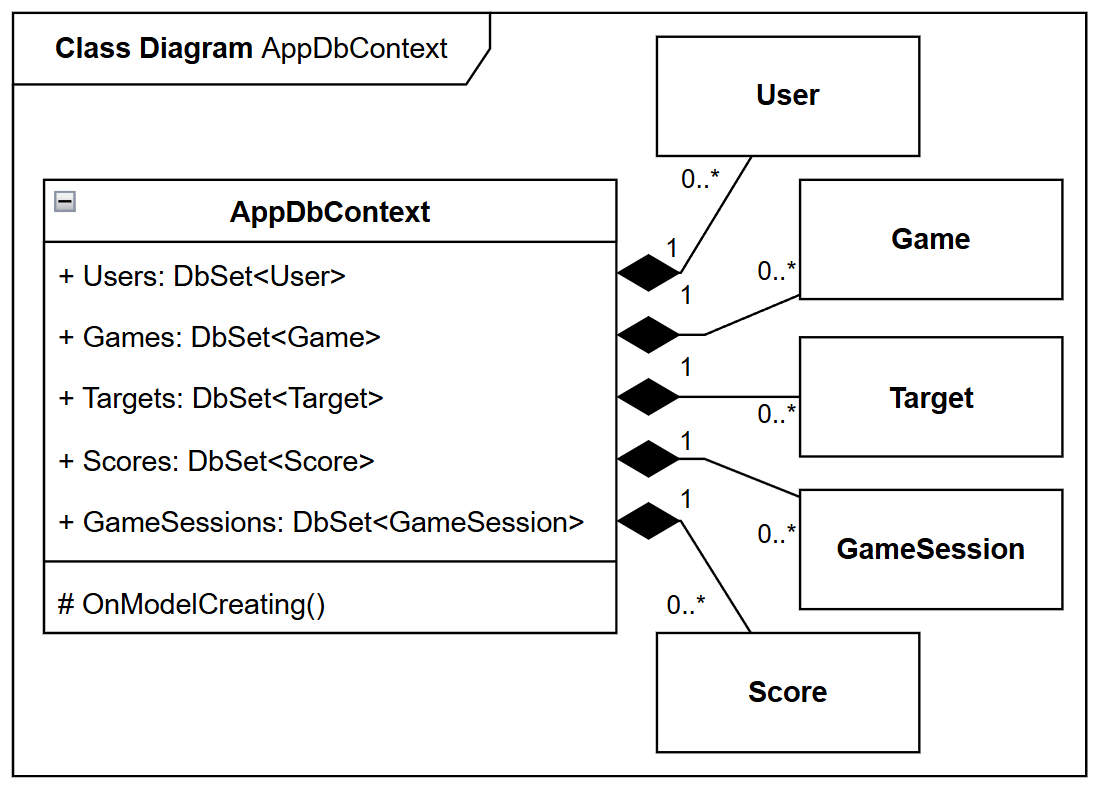
\includegraphics[width=0.6\textwidth]{images/AppDbClass.png}
        \caption{AppDbContext klasių diagrama (Loginis pjūvis)}
        \label{fig:appdb}
    \end{figure}
\end{frame}

\begin{frame}{Privačių ir viešų žaidimų kūrimo klasių diagrama (Loginis pjūvis)}
    \begin{figure}[H]
        \centering
        
\includegraphics[width=0.5\textwidth]{images/GameCreationClassImg.png}
        \caption{Privačių ir viešų žaidimų kūrimo klasių diagrama (Loginis pjūvis)}
        \label{fig:gamecreation}
    \end{figure}
\end{frame}

\begin{frame}{Geriausių rezultatų ir lyderių lentelė (Loginis pjūvis)}
    \begin{figure}[H]
        \centering
        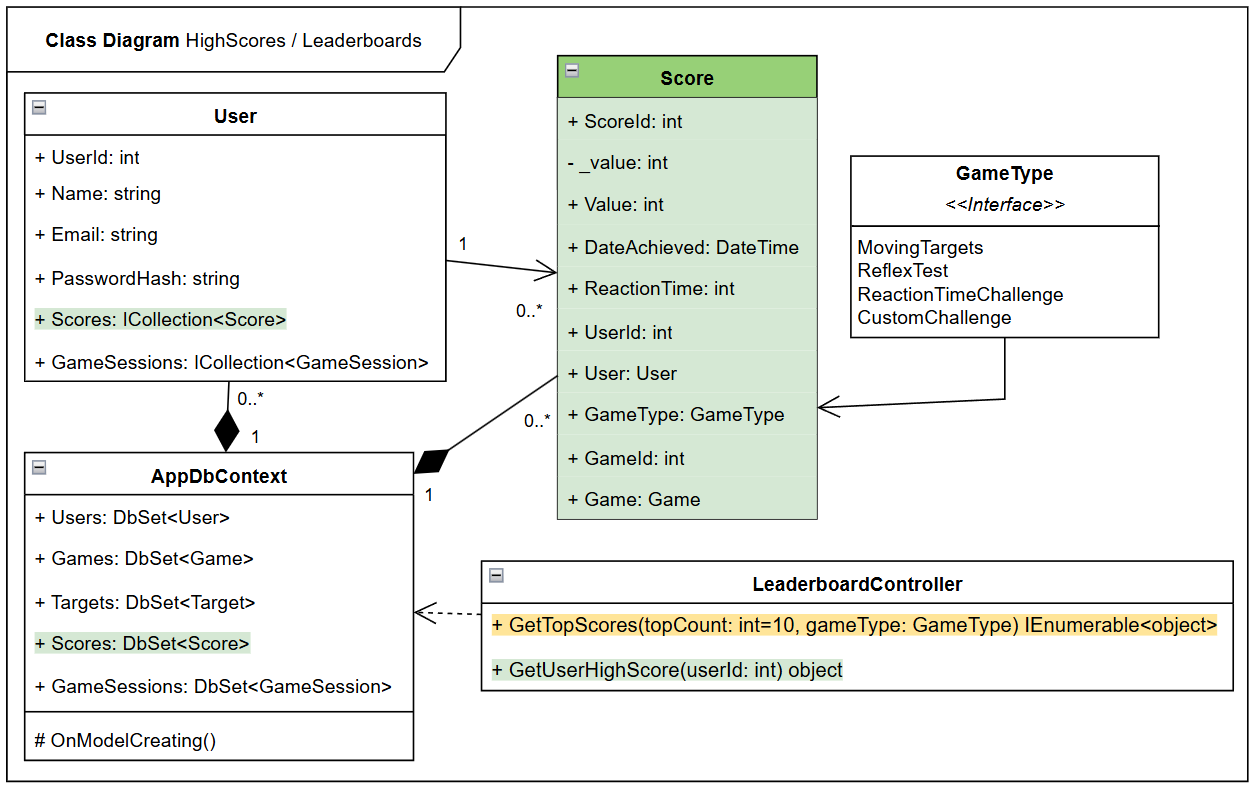
\includegraphics[width=0.7\textwidth]{images/highLeadClass.png}
        \caption{Geriausių rezultatų ir lyderių lentelės klasių diagrama (Loginis pjūvis)}
        \label{fig:leaderboard}
    \end{figure}
\end{frame}

\begin{frame}{Žaidimų istorija (Loginis pjūvis)}
    \begin{figure}[H]
        \centering
        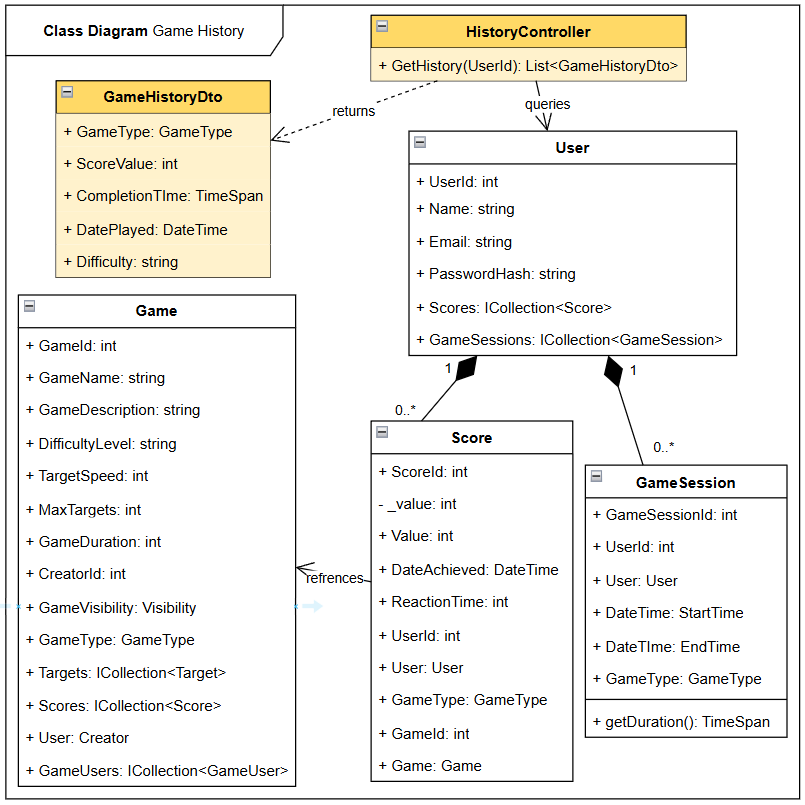
\includegraphics[width=0.55\textwidth]{images/clasNEWGameHistory.png}
        \caption{Žaidimų istorijos klasių diagrama (Loginis pjūvis)}
        \label{fig:gameHistory}
    \end{figure}
\end{frame}

\begin{frame}{Žaidimų vertinimas (Loginis pjūvis)}
    \begin{figure}[H]
        \centering
        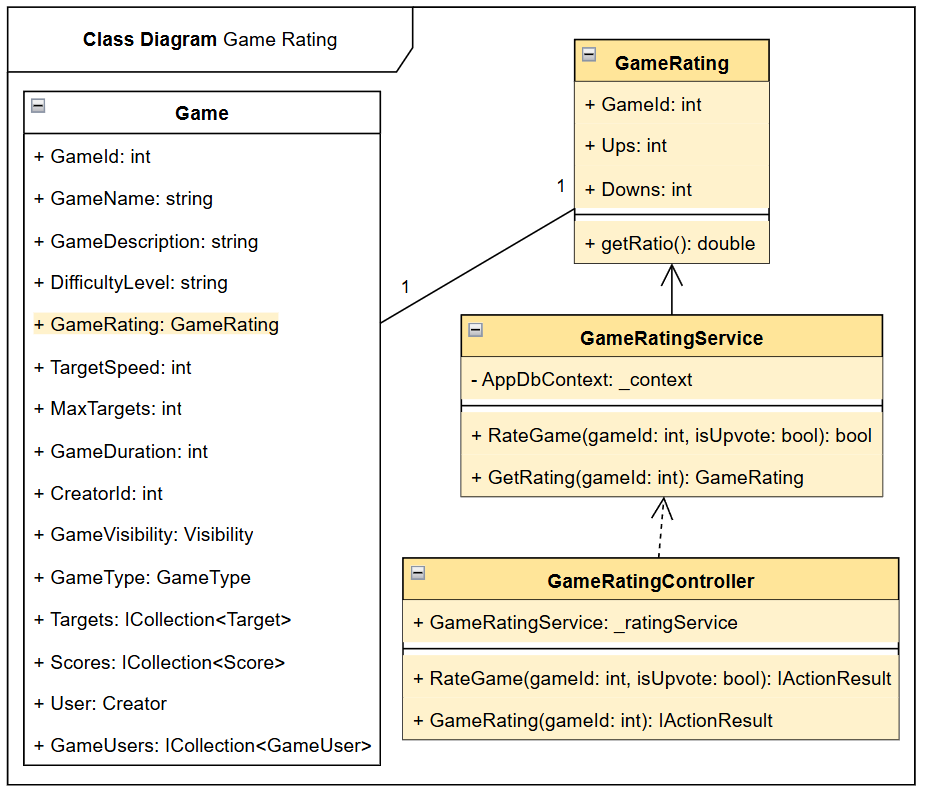
\includegraphics[width=0.6\textwidth]{images/gameRatingClassNEW.png}
        \caption{Žaidimų vertinimo klasių diagrama (Loginis pjūvis)}
        \label{fig:gameRating}
    \end{figure}
\end{frame}

\begin{frame}{Viešų žaidimų kūrimo sekos diagrama (Proceso pjūvis)}
    \begin{figure}[H]
        \centering
        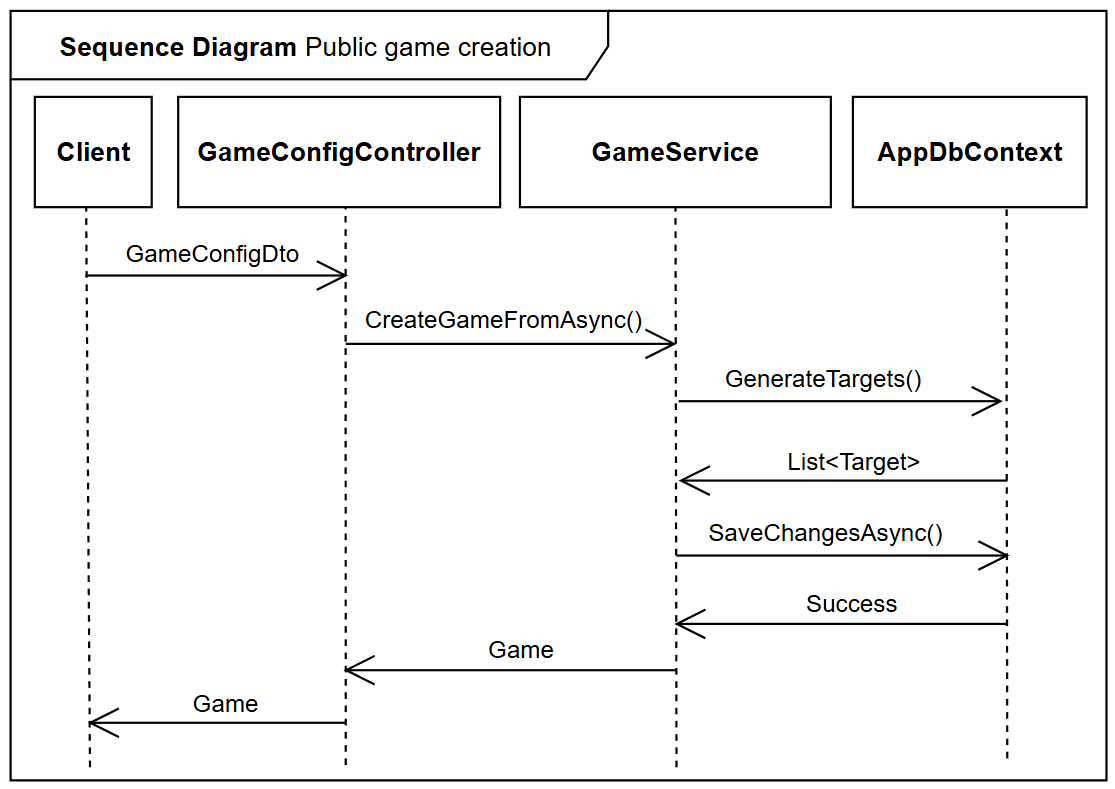
\includegraphics[width=0.6\textwidth]{images/seqPublic.png}
        \caption{Viešų žaidimų kūrimo sekos diagrama (Proceso pjūvis)}
        \label{fig:privseq}
    \end{figure}
\end{frame}

\begin{frame}{Privačių žaidimų kūrimo sekos diagrama (Proceso pjūvis)}
    \begin{figure}[H]
        \centering
        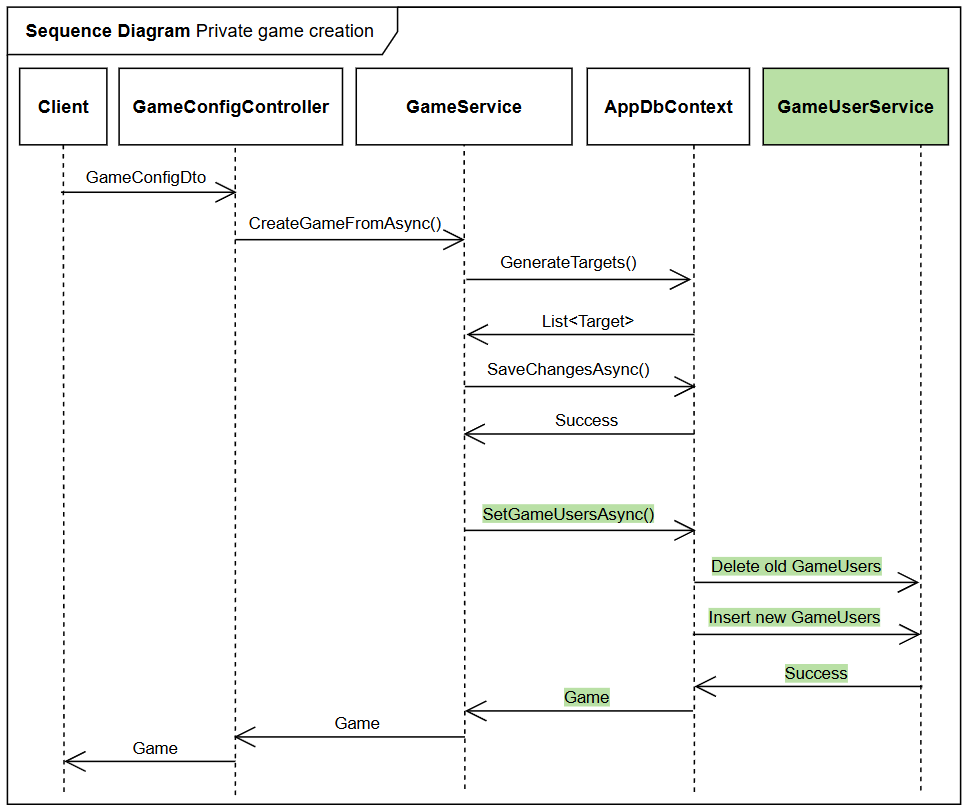
\includegraphics[width=0.6\textwidth]{images/seqPrivate.png}
        \caption{Privačių žaidimų kūrimo sekos diagrama (Proceso pjūvis)}
        \label{fig:pubseq}
    \end{figure}
\end{frame}

\begin{frame}{Žaidimų vertinimo sekos diagrama (Proceso pjūvis)}
    \begin{figure}[H]
        \centering
        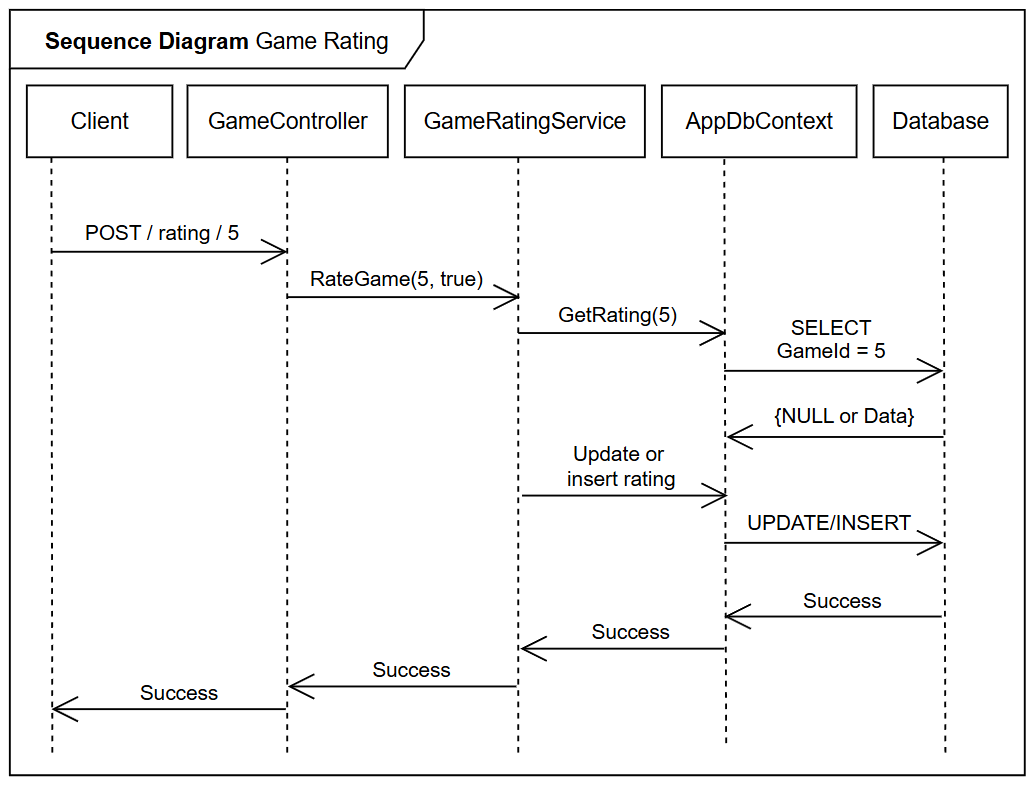
\includegraphics[width=0.6\textwidth]{images/sqgameRating.png}
        \caption{Žaidimų vertinimo sekos diagrama (Proceso pjūvis)}
        \label{fig:gameRatingSeq}
    \end{figure}
\end{frame}

\begin{frame}{Privačių ir viešų žaidimų kūrimo veiklos diagrama (Panaudojimo atvejų pjūvis)}
    \begin{figure}[H]
        \centering
        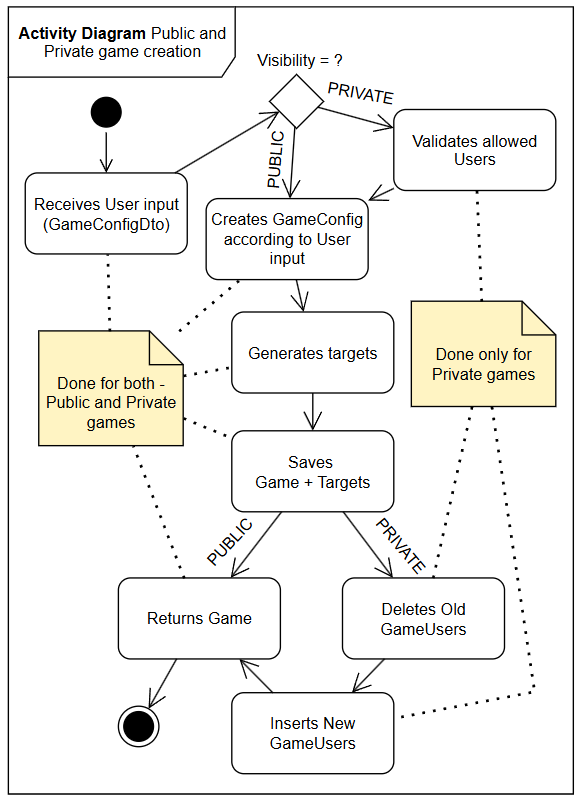
\includegraphics[width=0.3\textwidth]{images/activPrivPubl.png}
        \caption{Supaprastinta privačių ir viešų žaidimų kūrimo veiklos diagrama (Panaudojimo atvejų pjūvis)}
        \label{fig:privpubactivity}
    \end{figure}
\end{frame}

\begin{frame}{Lyderių lentelės veiklos diagrama (Panaudojimo atvejų pjūvis)}
    \begin{figure}[H]
        \centering
        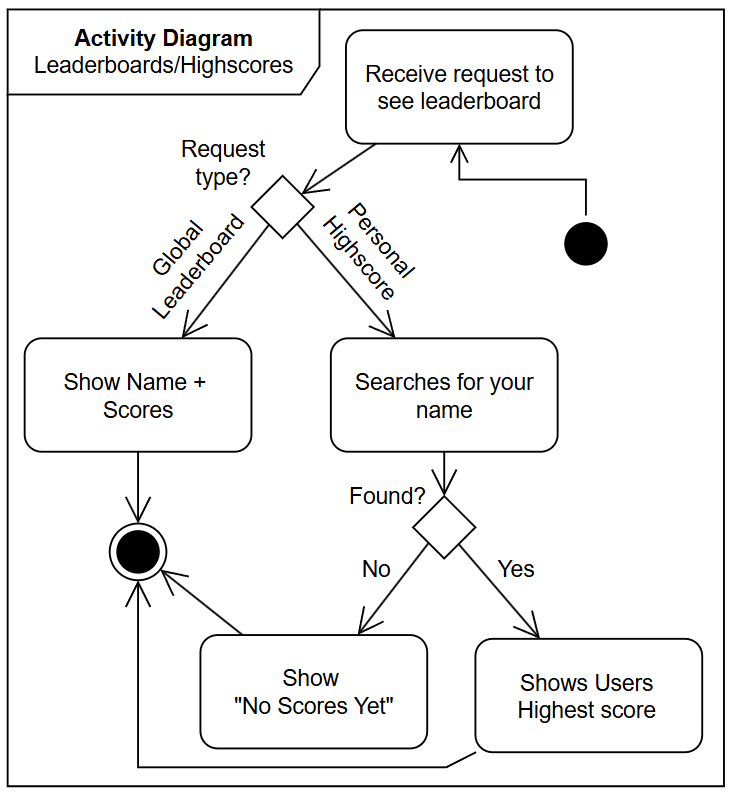
\includegraphics[width=0.4\textwidth]{images/leaderHighAct.png}
        \caption{Lyderių lentelės veiklos diagrama (Panaudojimo atvejų pjūvis)}
        \label{fig:leaderhighactivity}
    \end{figure}
\end{frame}

\begin{frame}{Žaidimų istorijos veiklos diagrama (Panaudojimo atvejų pjūvis)}
    \begin{figure}[H]
        \centering
        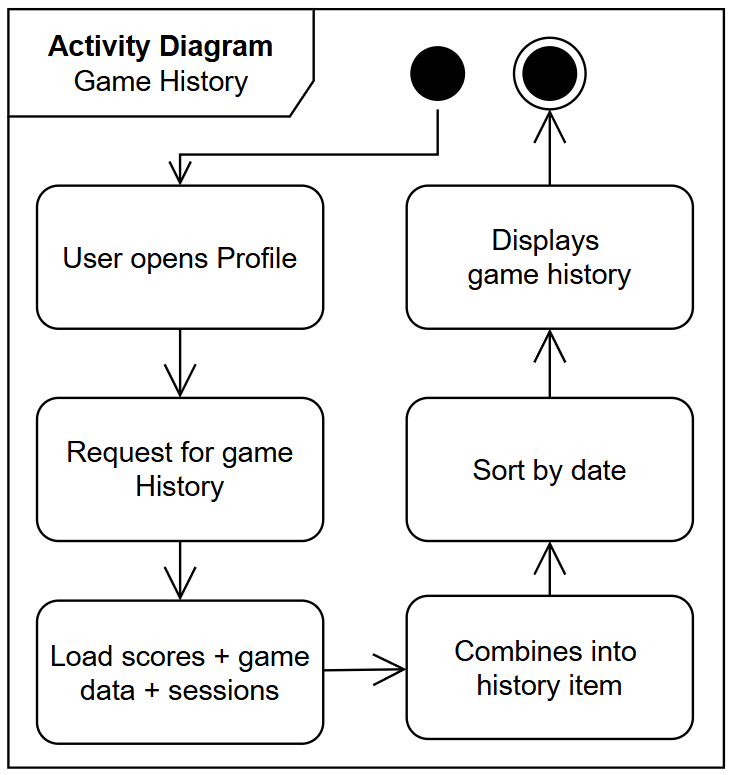
\includegraphics[width=0.4\textwidth]{images/gameHistoryAct.png}
        \caption{Žaidimų istorijos veiklos diagrama (Panaudojimo atvejų pjūvis)}
        \label{fig:gamehistoryactivity}
    \end{figure}
\end{frame}


\begin{frame}{Komponentų diagrama 1 (Kūrimo pjūvis)}
    \begin{figure}[H]
    \centering
    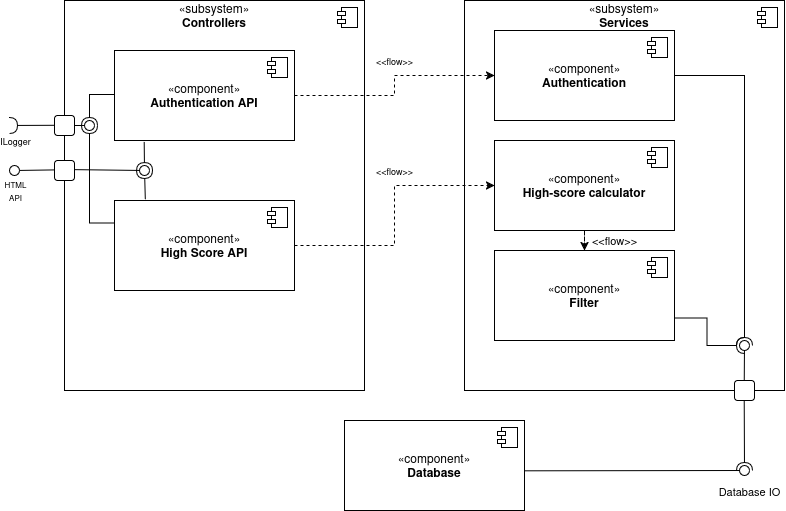
\includegraphics[width=0.8\textwidth]{images/Arno/highscoresandleaderboardF.drawio.png}
    \caption{Komponentų diagrama (Geriausi rezultatai ir lyderių lentelė)}
    \label{fig:component-diagram 4}
    \end{figure}
\end{frame}

\begin{frame}{Komponentų diagrama 2 (Kūrimo pjūvis)}
   \begin{figure}[H]
    \centering
    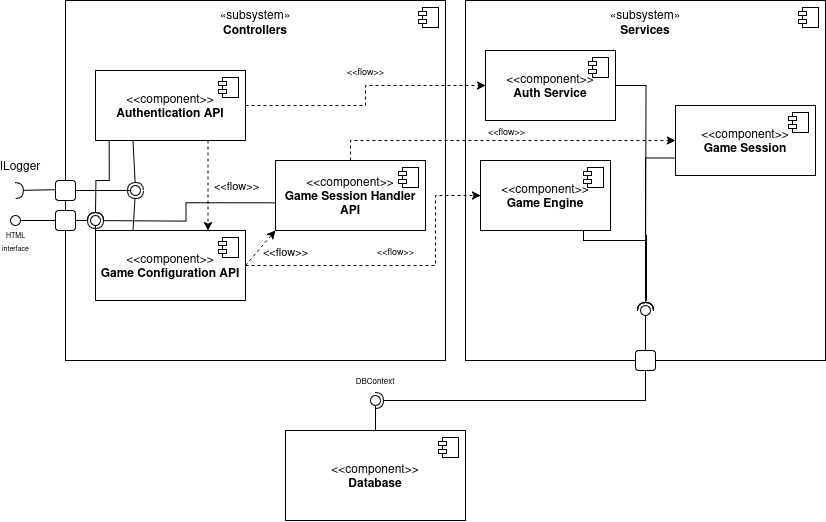
\includegraphics[width=0.8\textwidth]{images/Arno/Component diagramF.drawio.png}
    \caption{Komponentų diagrama (Kelių žaidėjų ir privatūs žaidimai)}
    \label{fig:component-diagram 1}
\end{figure}
\end{frame}
\begin{frame}{Komponentų diagrama 3 (Kūrimo pjūvis)}
   \begin{figure}[H]
    \centering
    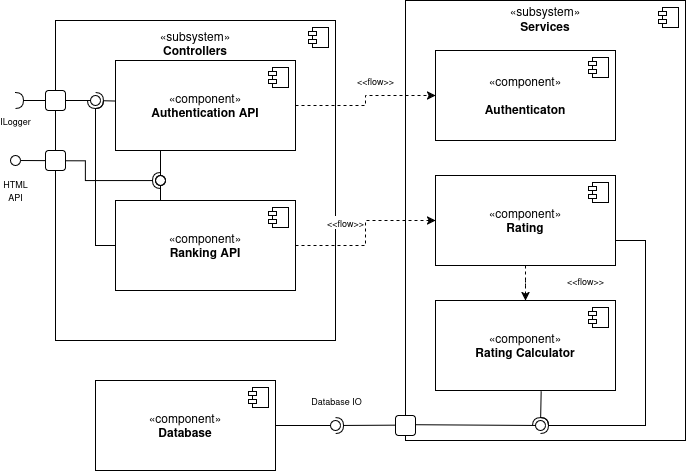
\includegraphics[width=0.8\textwidth]{images/Arno/RankingF.drawio.png}
    \caption{Komponentų diagrama (Vertinimo sistema)}
    \label{fig:component-diagram 2}
    \end{figure}
\end{frame}
\begin{frame}{Komponentų diagrama 4 (Kūrimo pjūvis)}
    \begin{figure}[H]
    \centering
    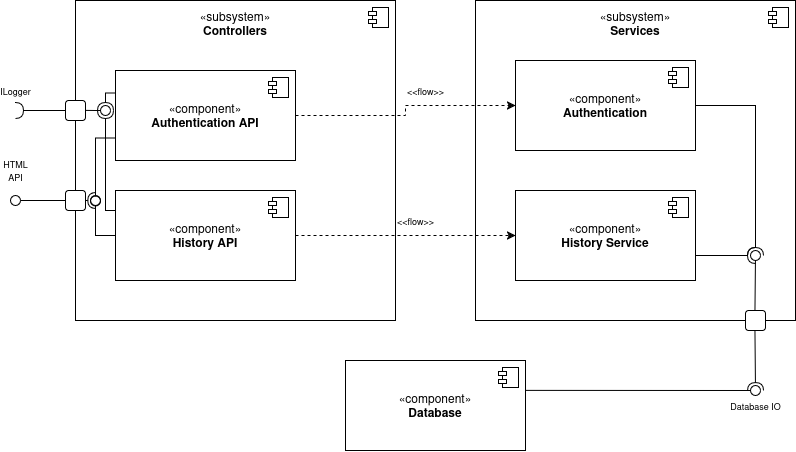
\includegraphics[width=0.8\textwidth]{images/Arno/GameHistoryF.drawio.png}
    \caption{Komponentų diagrama (Žaidimų istorija)}
    \label{fig:component-diagram 3}
    \end{figure}
\end{frame}
\begin{frame}{Paketų diagrama (Kūrimo pjūvis)}
   \begin{figure}[H]
    \centering
    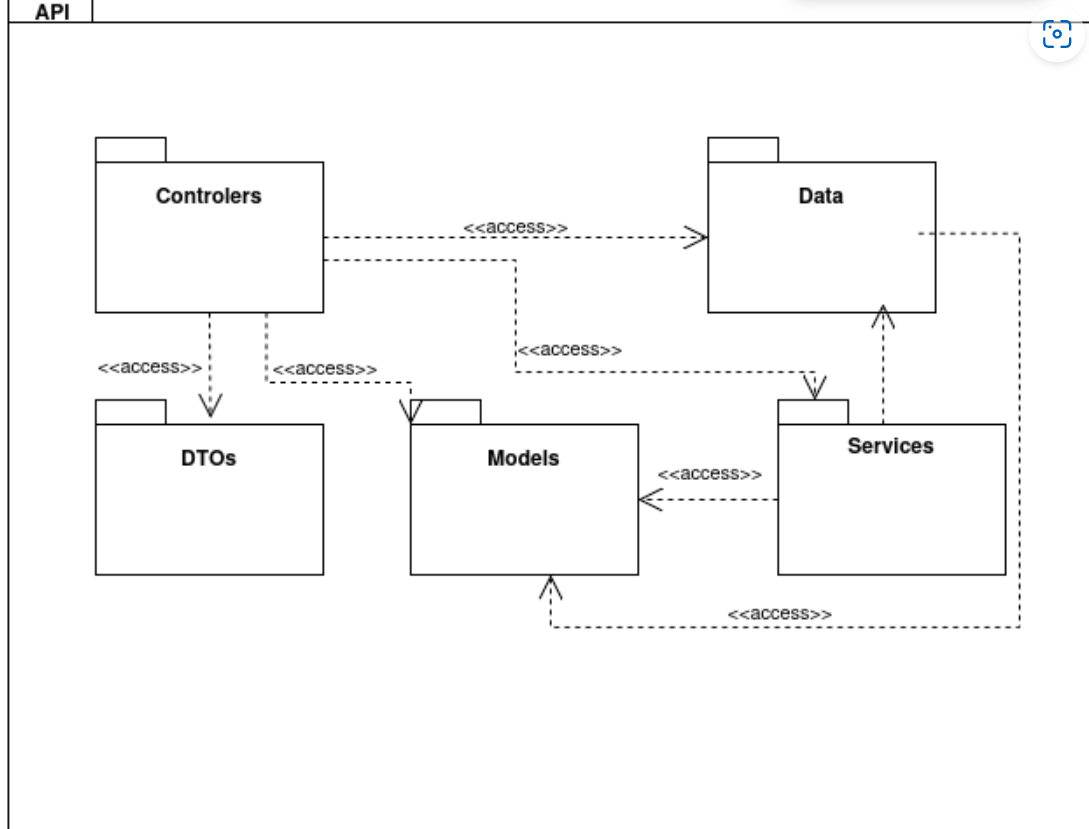
\includegraphics[width=0.8\textwidth]{images/Arno/package.png}
    \caption{Paketų diagrama (Kūrimo pjūvis)}
    \label{fig:package-diagram}
    \end{figure}
\end{frame}
\begin{frame}{Artefaktų diagrama 1 (Fizinis pjūvis)}
    \begin{figure}[H]
        \centering
        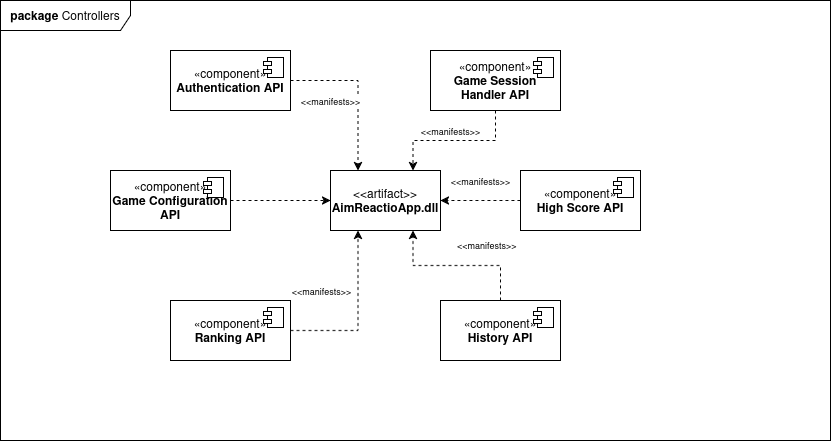
\includegraphics[width=0.8\textwidth]{images/Arno/ArtifactsControllersW.drawio.png}
        \caption{Artefaktų diagrama (Valdiklių artefaktai)}
        \label{fig:package-diagram}
    \end{figure}
\end{frame}
\begin{frame}{Artefaktų diagrama 2 (Fizinis pjūvis)}
   \begin{figure}[H]
    \centering
    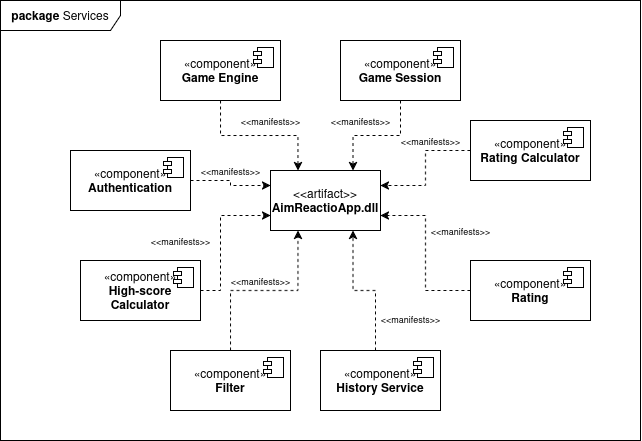
\includegraphics[width=0.8\textwidth]{images/Arno/ArtifactsServicesW.drawio.png}
    \caption{Artefaktų diagrama (Paslaugų artefaktai)}
    \label{fig:package-diagram}
    \end{figure}
\end{frame}
\section{CI/CD}





\begin{frame}{CI/CD 1 etapas}
    \begin{columns}[T] % Align columns to the top
        \column{0.5\textwidth} % Left column for the image
            \begin{figure}
                \includegraphics[width=\linewidth]{images/cicd/"stage 1.png"}
                \caption{1 etapas}
            \end{figure}
            \column{0.5\textwidth} % Right column for the text
            \textbf{1 etapo aprašymas:} \\
            Aplikacijos kompiliavimo komandos:
            \begin{itemize}
                \item \texttt{dotnet build}
                \item \texttt{npm run build}
            \end{itemize}
            Vidutinis laikas: 58s
            
            Programuotojas gali įtraukti \textbf{\#patch}, \textbf{\#minor}, \textbf{\#major} į įrašo pranešimą, kad automatiškai atnaujintų aplikacijos versiją.

    \end{columns}
\end{frame}

\begin{frame}{CI/CD 2-3 etapai}
    \begin{columns}[T] % Align columns to the top
        \column{0.5\textwidth} % Left column for the image
        \begin{figure}
            \includegraphics[width=\linewidth]{images/cicd/"stage 2-3.png"}
            \caption{2-3 etapai}
        \end{figure}
        \column{0.5\textwidth} % Right column for the text
        \textbf{2 etapo aprašymas:} \\
        Aplikacijos testavimo komandos:
        \begin{itemize}
            \item \texttt{dotnet test}
            \item \texttt{npm run test}
        \end{itemize}
        Vidutinis laikas: 37s
        
        Vitest ir NUnit naudojami frontendo ir backendo testavimui. 
    \end{columns}
\end{frame}

\begin{frame}{CI/CD 2-3 etapai}
    \begin{columns}[T] % Align columns to the top
        \column{0.5\textwidth} % Left column for the image
        \begin{figure}
            \includegraphics[width=\linewidth]{images/cicd/"stage 2-3.png"}
            \caption{2-3 etapai}
        \end{figure}
        \column{0.5\textwidth} % Right column for the text
        \textbf{3 etapo aprašymas:} \\
        Aplikacijos dockerizavimo komandos:
        \begin{itemize}
            \item \texttt{docker build -t frontend-app .}
            \item \texttt{docker build -t backend-app .}
        \end{itemize}
        Vidutinis laikas: 17s

        Maksimalus laikas: 87s

        Minimalus laikas: 6s
    \end{columns}
\end{frame}

\begin{frame}{CI/CD 4-5 etapai}
    \begin{columns}[T] % Align columns to the top
        \column{0.5\textwidth} % Left column for the image
        \begin{figure}
            \includegraphics[width=\linewidth]{images/cicd/"stage 4-5.png"}
            \caption{4-5 etapai}
        \end{figure}
        \column{0.5\textwidth} % Right column for the text
        \textbf{4 etapo aprašymas:} \\
        Duomenų bazės atnaujinimo komanda:
        \begin{itemize}
            \item \texttt{dotnet ef database update}
        \end{itemize}
        Vidutinis laikas: 14s

        Programuotojas privalo įtraukti \textbf{\#migration} į įrašo pranešimą, kad suaktyvintų šį etapą.
    \end{columns}
\end{frame}

\begin{frame}{CI/CD 4-5 etapai}
    \begin{columns}[T] % Align columns to the top
        \column{0.5\textwidth} % Left column for the image
        \begin{figure}
            \includegraphics[width=\linewidth]{images/cicd/"stage 4-5.png"}
            \caption{4-5 etapai}
        \end{figure}
        \column{0.5\textwidth} % Right column for the text
        \textbf{Aprašymas:} \\
        Diegimo komanda:
        \begin{itemize}
            \item \texttt{docker-compose up -d}
        \end{itemize}
        Vidutinis laikas: 8s
    \end{columns}
\end{frame}




\begin{frame}{Diegimo aplinka (Fizinis pjūvis)}
    \begin{figure}
        
\includegraphics[width=0.8\linewidth]{images/cicd/DeploymentEnv.drawio.png}
        \caption{Diegimo aplinka}
    \end{figure}
\end{frame}

\begin{frame}{Produkcijos diagrama (Fizinis pjūvis)}
    \begin{figure}
        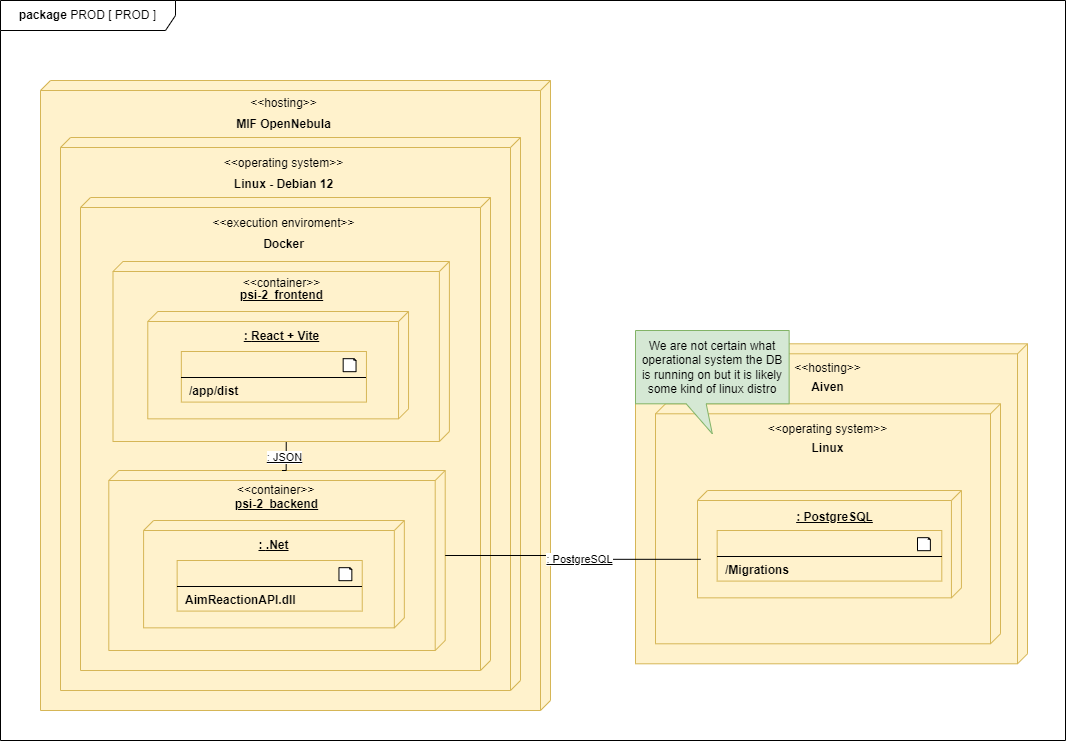
\includegraphics[width=0.65\linewidth]{images/cicd/PROD Diagram.drawio.png}
        \caption{Produkcijos diagrama}
    \end{figure}
\end{frame}




\begin{frame}{Išteklių poreikiai}
    Duomenų bazės išteklių poreikiai:
    \begin{table}[H]
        \centering
        \begin{tabular}{|c|c|c|}
            \hline
            \textbf{Reikalavimo tipas} & \textbf{Minimalūs reikalavimai} & \textbf{Rekomenduojami reikalavimai} \\ 
            \hline
            Duomenų bazės CPU & 1 branduolys & 1 branduolys \\ 
            \hline
            Duomenų bazės RAM & 1 GB & 1 GB \\ 
            \hline
            Duomenų bazės talpa & 1 GB & 5 GB \\ 
            \hline
        \end{tabular}
        \caption{Sistemos reikalavimai duomenų bazei}
        \label{tab:system-requirements}
    \end{table}
\end{frame}

\begin{frame}{Išteklių poreikiai}
    Įrenginio išteklių poreikiai:
    \begin{table}[H]
        \centering
        \begin{tabular}{|c|c|c|}
            \hline
            \textbf{Ištekliaus tipas} & {Minimalūs poreikiai} & {Rekomenduojami} \\ 
            \hline
            Talpa & 6 GB & 10 GB \\ 
            \hline
            RAM & 1 GB & 2 GB \\ 
            \hline
            CPU & 0.4 branduolio & 1 branduolys \\ 
            \hline
            Įkėlimas & 629 Mbit/s & 1 Gbit/s \\
            \hline
            Atsisiuntimas & 8 Mbit/s & 200 Mbit/s \\
            \hline
            Tinklo vėlinimas & ≈30 ms & ≈10 ms \\
            \hline
        \end{tabular}
        \caption{Įrenginio išteklių poreikiai}
        \label{tab:resource-types}
    \end{table}
\end{frame}


%------------------------------------------------

\begin{frame}
    \Huge{\centerline{\textbf{Demo}}}
\end{frame}

%----------------------------------------------------------------------------------------

\end{document}